\documentclass{standalone}

\usepackage{tikz}
\usetikzlibrary{calc}
\begin{document}

% TANGENT to CIRCLE - known: r, q
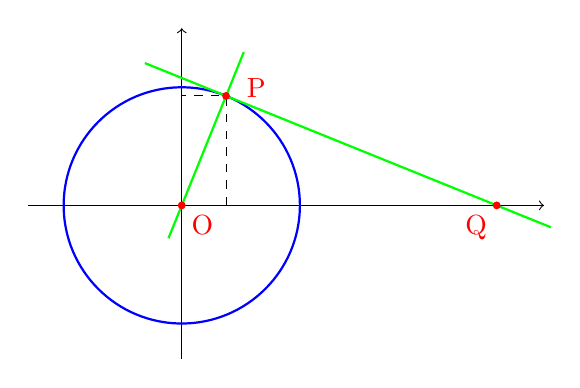
\begin{tikzpicture}
  \def\r{1.5} % radius
  \def\q{4} % distance center-external point q = |OQ|
  \def\x{{\r^2/\q}} % Q x coordinate
  \def\y{{\r*sqrt(1-(\r/\q)^2}} % Q y coordinate
  \coordinate (O) at (0,0); % circle center O
  \coordinate (Q) at (\q,0); % external point Q
  \coordinate (P) at (\x,\y); % point of tangency, P
  \draw[->] (0,-1.3*\r) -- (0,1.5*\r);
  \draw[->] (-1.3*\r,0) -- (\q+0.4*\r,0);
  \draw[dashed] (\x,0) |- (0,\y);
  \draw[blue,thick] (O) circle(\r);
  \draw[green,thick] ($(Q)!-0.2!(P)$) -- ($(Q)!1.3!(P)$);
  \draw[green,thick] ($(O)!-0.3!(P)$) -- ($(O)!1.4!(P)$);
  \fill[red] (O) circle(0.05) node[below right] {O};
  \fill[red] (Q) circle(0.05) node[below left] {Q};
  \fill[red] (P) circle(0.05) node[above=3,right=4] {P};
\end{tikzpicture}

% TANGENT to ELLIPSE - known: a, b, q
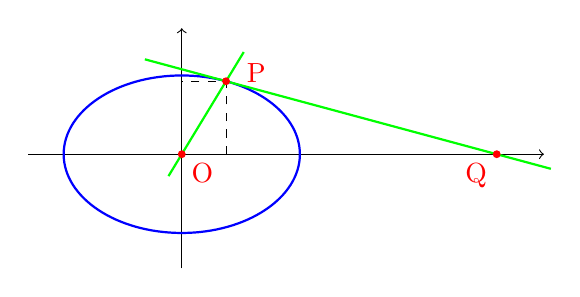
\begin{tikzpicture}
  \def\a{1.5} % horizontal radius
  \def\b{1.0} % vertical radius
  \def\q{4} % distance center-external point q = |OQ|
  \def\x{{\a^2/\q}} % x coordinate P
  \def\y{{\b*sqrt(1-(\a/\q)^2}} % y coordinate P
  \coordinate (O) at (0,0); % circle center O
  \coordinate (Q) at (\q,0); % external point Q
  \coordinate (P) at (\x,\y); % point of tangency, P
  \draw[->] (0,-\b-0.3*\a) -- (0,\b+0.4*\a);
  \draw[->] (-1.3*\a,0) -- (\q+0.4*\a,0);
  \draw[dashed] (\x,0) |- (0,\y);
  \draw[blue,thick] (O) ellipse({\a} and {\b});
  \draw[green,thick] ($(Q)!-0.2!(P)$) -- ($(Q)!1.3!(P)$);
  \draw[green,thick] ($(O)!-0.3!(P)$) -- ($(O)!1.4!(P)$);
  \fill[red] (O) circle(0.05) node[below right] {O};
  \fill[red] (Q) circle(0.05) node[below left] {Q};
  \fill[red] (P) circle(0.05) node[above=3,right=4] {P};
\end{tikzpicture}

\end{document}




